\chapter{Implementation}\label{chap:implementation}

 The aim of the thesis was not only to get the basic understanding of an NLG process, but also to try to create the implementation in a language that is widely used around the world: Python.  The goal was to create an end-to-end NLG system, that takes non-processed raw data about a football match as an input and creates an article in Czech language that summarises the course of the match. In this chapter we will take a closer look at the overall functioning of the football articles generating NLG system.

\section{Requirements and initial goal}
As mentioned in the introduction of this section, the expected output was simply a readable Czech text summary while attempting to produce sentences that are not identical, resulting in a less-monotonic text. Since the expected output was defined somewhat vague and quality-wise uncertain, there is no stress on the definition of the goal of the language as well as target audience. However, the text quality, especially in the variability of expressions, used structures and overall richness, is insufficient to truly satisfy the definition of an (newspaper) article. 

Since NLG is a complex process we used one already existing tool for linguistic realisation - \emph{Genja API} by Geneea. Without this system the output language would not be grammatically correct and therefore not satisfying the readability requirement. As discussed in \ref{section:lr} this task has no easy way of implementing manually, especially not for a Czech language that belongs to the most complicated natural languages (for reasons that are described in \ref{section:lr} as well). \emph{Genja API} usage skips this task focusing on the rest of the NLG tasks.

In \autoref{chap:process} we proposed an outline to a requirements analysis. This chapter tries to follow this structure discussing and describing the specifics of each segment. Unluckily, in order to present the closely-connected requirements and their consequences in a organised way, we may modify the structure slightly.

\section{Input data}
The dataset was provided by the company Livesport s.r.o. (see \url{https://www.livesport.cz/}), which I would like to thank. Therefore the entire dataset can not be shared. However, one example match is attached to illustrate program functioning. Initial dataset is composed of every match of one Czech First League season. Every match is represented as a JSON file storing both general information about the match (teams, venue, attendance, line-ups, etc.) and course of key events of the matches (goals, substitutions, cards, etc.). 

General information about the match consists of two participating teams, starting time of the match, tournament information (here Czech First League, season 2018/2019), information about venue, score, winner, stage of the game (e.g. finished/delayed) and line-up. Line-up consists of every player of the team divided into groups according to their status (e.g. injured, benched, initial line-up, etc.) along with other information like home country, number and more. 

Course of events is represented as a list of incidents. Incidents have attributes like id, time, participant, type and so on. Also, incidents have attribute \emph{parentId}, which further specifies the incident. For instance incident type \emph{Penalty Kick} has empty \emph{parentId}, however, in the list of incidents there is an incident with the type of \emph{Penalty Scored} or \emph{Penalty Missed} that has \emph{parentId} identical to the corresponding \emph{Penalty Kick} incident \emph{Id}. 

Detailed examples of the representation of the input data are shown later in \figref{player} and \figref{incident}.

\section{Approach}

For this particular NLG problem we have chosen modular architecture as described in \ref{section:modules}: the most traditional, even though now a little outdated, approach proposed by \cite {reiter1997building} consisting of grouping similar NLG tasks into modules that are then connected via one-way-pipeline. 

In the first place, we would like to highlight the core reasons that led to a chosen approach:
\begin{itemize}
	\item My personal lack of experience in NLG as this was my first ever NLG system that I have created.
	\item The lack of easily accessible high amount of data.
	\item The full extent of an NLG problem: from non-processed data to well-built text.   
\end{itemize}

For me, personally, this field of computational linguistics is new and therefore the aim  was not only to build a NLG system, but to gain knowledge including different approaches in this specific subfield of NLP. Personally, staying faithful to the division of modules is the most intuitive and also feasible solution, which closely relates to the point of the end-to-end extent of the problem. It was easy for me to get lost in the high amount of issues to resolve (each of the NLG tasks) without giving it a properly organised structure. The lack of experience also resulted in the error propagation that has risen repeatedly during the development. 

In addition, the lack of data almost forbids the data-driven approach. Naturally, the data do exist, but their acquisition would require either a high amount of time-consuming labour of creating the data by hand or acquiring football articles automatically and then aligning them with given input data, which still can end up insufficient as for the acquired text more data could have been known. Such a corpus building could be a project on its own.

\section{Match example}
A match example is provided and the summary can be seen in \figref{overview}. 

Football match between \emph{Jablonec} and \emph{Bohemians 1905}, which resulted in a 3 to 1 victory for the home team \emph{Jablonec}. First half can be summarised into words to further describe the figure as follows: First goal was a penalty scored by \emph{Trávník} in 10th minute and then second incident was a goal by \emph{Bohemians'} player \emph{Hašek} that tied the game in 44th minute after a pass from \emph{Vaníček}. Events that happened in the second half are hopefully easy to interpret as well. Numbers next to an incident group them by their type- (1) penalty goal, (2) goal with an assist, (3) substitution and (4) yellow card. 

\begin{figure}[H]
	\centering{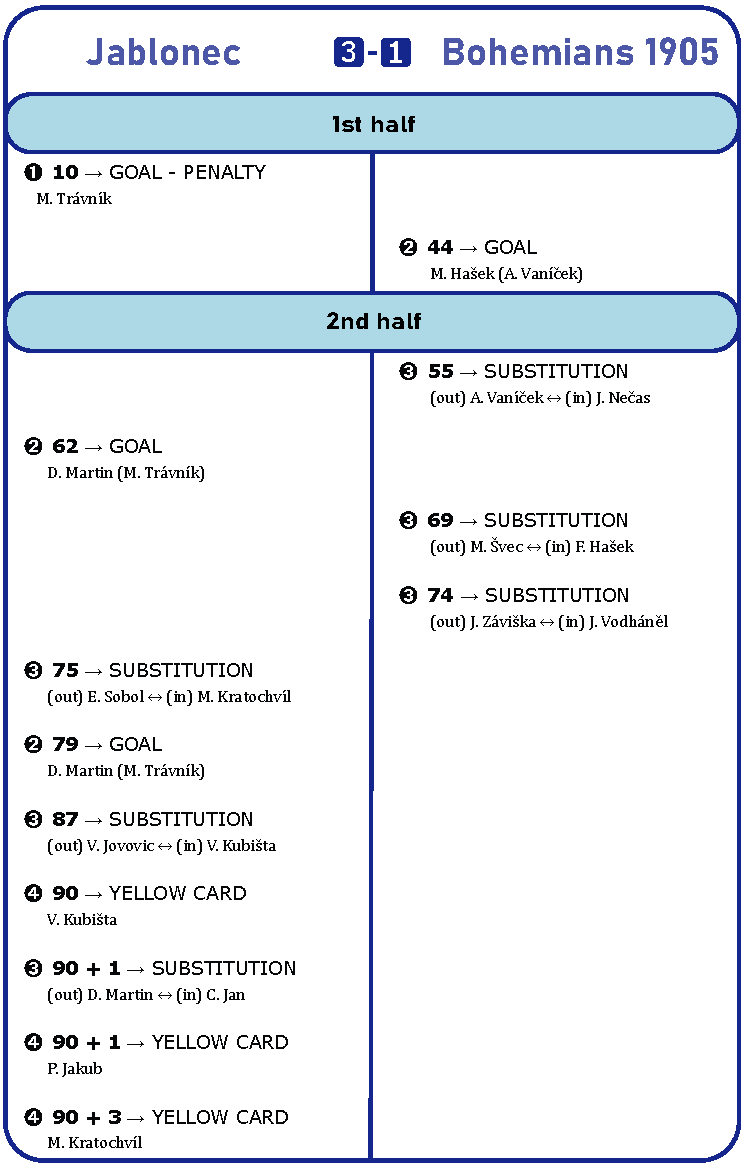
\includegraphics[width=0.93\textwidth]{./img/match_overview.pdf}}
	\caption{Table summary of the example match.}
	\label{fig:overview}
\end{figure}

\section{Structure overview}
The overview of the structure of the solution is shown in \figref{structure}.

Input data with arguments to modify slight functioning (as a way of output is presented, number of texts to generate, input data or key for Genja) are passed to \emph{run.py} (\figref{structure} - 1) (.py will be left out as it is implicit for every module), which is the executable starting point of the program. Parsed arguments are an input for \emph{articles\_generator}, which handles the communication between each module, essentially creating the one-way-pipeline for modules (\figref{structure} - 2, 3, 4, 5) and managing passing correct arguments to functions. Output of this core handler is tuple of strings: title and body of the article.

The \emph{data\_initializer} (\figref{structure} - 2) module is not present in the original modular architecture by \cite{reiter1997building} (described in \ref{section:modules}). However, since the data are in a raw form, the step of data processing needed to be added to store the data internally in a more convenient way to further operate with the information given effectively.

Modules (\figref{structure} - 3, 4, 5) correspond to the modular architecture perfectly. \emph{Document\_planner} (\figref{structure}-3) takes data about a match in a convenient inner representation as an input and creates a \emph{DocumentPlan}, which contains ordered preverbal messages to be said in an article. Then these messages are lexicalized in \emph{sentence\_planner} (\figref{structure} - 4) and finally linguistically realised by \emph{linguistic\_realiser} (\figref{structure} - 5). 

Moreover, there are three auxiliary modules (described in detail in \ref{subsection:aux}) to keep the structure of the modular approach implementation as clean as possible:
\begin{itemize}
	\item \emph{Data.py}
	\item \emph{Types.py}
	\item \emph{printer.py}
\end{itemize}

\begin{figure}[H]
	\centering{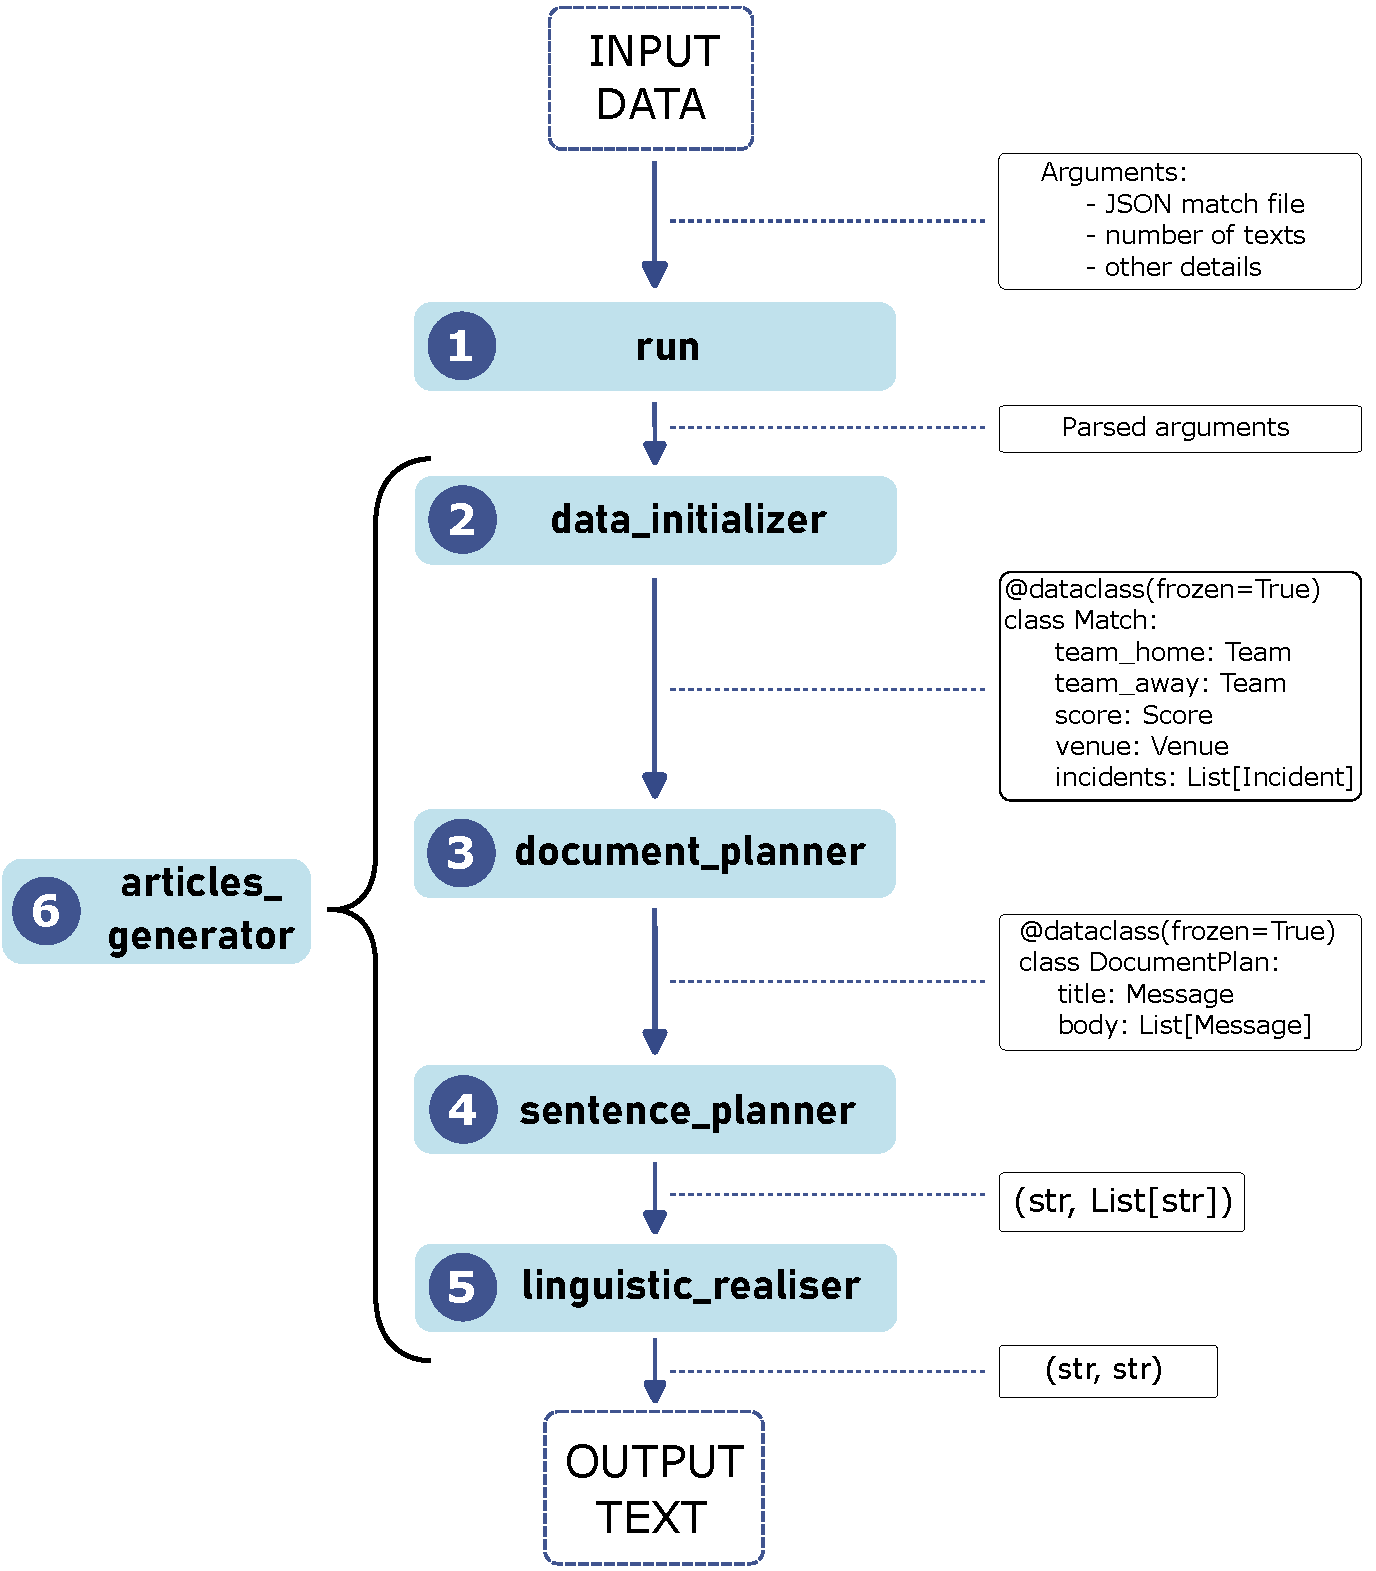
\includegraphics[width=1\textwidth]{./img/program_structure.pdf}}
	\caption{Overview of solution structure.}
	\label{fig:structure}
\end{figure}

\section{Modules implementation}
In this section the implementation of each module is described in detail creating a compact solution in Python. For even closer inspection, feel free to look into the code.

\subsection{Auxiliary modules}\label{subsection:aux}
\textbf{\textit{Data.py}} groups data classes that store information contained in a JSON file. Namely these entities are \emph{Score, Venue, Country, Player, Team, Time, Incident (+IncidentParent)} and finally the most crucial \emph{Match} that encapsulates each of the classes mentioned. Note that these classes are made immutable using \emph{@dataclass(frozen=True)} from package \emph{dataclasses} and then implementing static \emph{create} method. Immutability ensures the data remain intact after manipulating with them frequently in multiple functions across modules. 

Module \textbf{\textit{printer.py}} manages printing different components in a readable way. Since there is a lot of data, even during the development it was more convenient to pretty-print separate results of modules instead of inspecting more nested and complicated states during debugging. Due to numerous alignments and length of string appending, a separate module was created to not overload other segments of the code.

Lastly, \textbf{\textit{Types.py}} stores enumerate types for different entities. For instance, in the \emph{document\_planner} module there is a class \emph{Message} to store attributes of a preverbal message. One of the attributes is the type of the message defined as \emph{Types.Message}. This class is implemented in \emph{Types.py} (along with other types, which have arisen so often that a separate module was created) as Python's \emph{enumerate()}. Options are \emph{GOAL, PENALTY\_KICK\_MISSED, CARD, SUBSTITUTION, RESULT}. To give one more example, message that reports a card incident has attribute storing the type of card in \emph{Types.Card} - \emph{YELLOW, RED\_AUTO, RED\_INSTANT} (distinguishing the difference between two yellow cards and instant red card - to highlight the severeness of the foul). Similarly, other types of different-level entities are stored. 

\subsection{Data initializer}\label{subsection: di}
Goal of the \textbf{\textit{Data\_initializer}} is to transform data from the initial JSON file to a more convenient inner representation implemented as a system of classes to uphold the principles of object-oriented programming resulting in a crisp and well-divided structure.

The implementation is straightforward - we use the built-in package \emph{json} to ease the manipulation with a JSON file while initializing classes from the \textbf{\textit{Data}} module. 

Two examples of specific records contained in the JSON file and their Python representation are shown in \figref{player} and \figref{incident}. 

\begin{figure}[h]
	\centering{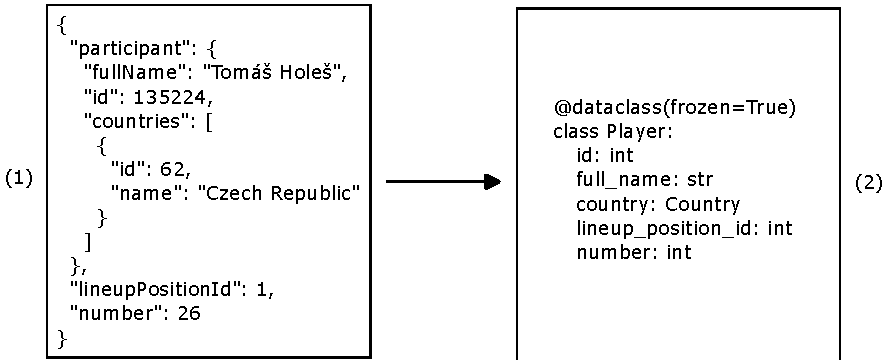
\includegraphics[width=0.9\textwidth]{./img/data_player.pdf}}
	\caption{Transformation of entity \emph{Player} from JSON to a Python class.}
	\label{fig:player}
\end{figure}

Entity {Player} is transformed from its initial JSON representation (\figref{player} - 1) to a easy-to-work-with Python's immutable class \emph{Player} with corresponding attributes. Note that a country has also a proper class \emph{Data.Country}.

\begin{figure}[h]
	\centering{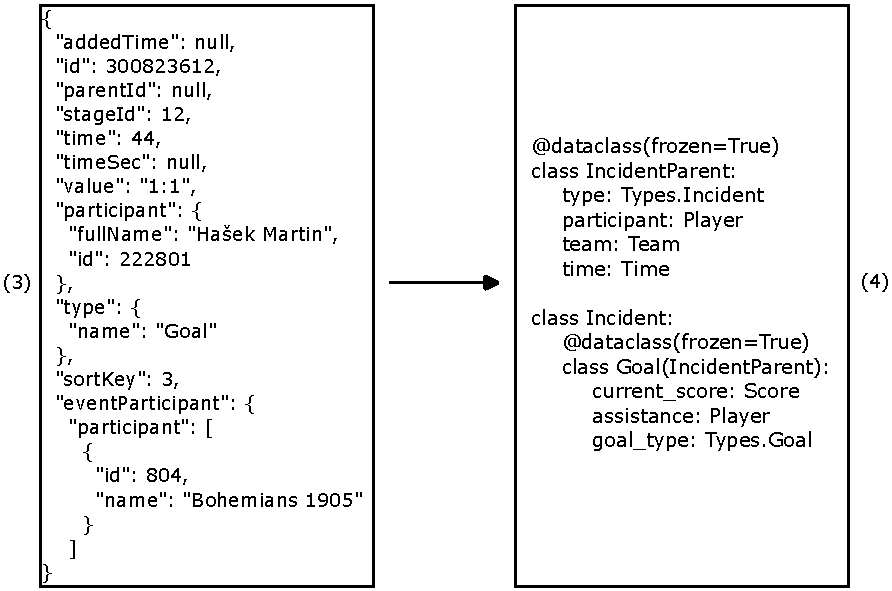
\includegraphics[width=1\textwidth]{./img/data_incident.pdf}}
	\caption{Transformation of entity \emph{Incident} from JSON to a Python class.}
	\label{fig:incident}
\end{figure} 

Entity \emph{Incident} is transformed from JSON (\figref{player} - 3) to a representation as an immutable Python's class (\figref{player} - 4). The class is called \emph{Goal} and it is a subclass of \emph{Incident}. This particular class structure ensures that different types of incidents (goal/card/substitution/penalty kick) can be addressed as one variable type and therefore enabling the \textit{Data.Match} class to have attribute \textit{incidents} storing incidents as \emph{List[Incident]}. Furthermore, every \textit{Incident} subclass also inherits from \emph{IncidentParent} class since these are common attributes for every match incident and it would be inefficient to repeat those attributes multiple times.

Note that this module resolves part of content determination since the number of attributes from the initial JSON file are not transformed into Python class. For instance, starting time of the match was not saved since we mark this information as redundant for an article generating. Similarly, more attributes were omitted to avoid useless information. On the other hand, couple attributes end up redundant (e.g. \textit{Country} of \textit{Player}), but these attributes are kept to ensure integrity of the solution and enable an easier further future development. 

\subsection{Document planner}

The aim of this module is to plan the content of the separate messages and their order. Document planner is resolved trivially - each incident is transformed to a separate preverbal message along with fundamental data. 

Implementation is shown in \figref{message} and is similar to \textit{Incident} structure. Each preverbal message has different arguments and therefore its own class. To access \textit{messages} classes as one variable type there is a system of inheritance, where every message class inherits from \textit{MessageParent} so that they can be distinguished by their according type \textit{Types.Message}. Note that these classes are made again immutable to ensure data stability.

Unlike message class \textit{Substitution}, which is self-explanatory, classes \textit{Result} and \textit{MissedPenalty} need clarification. 

\textit{Result} message defines the title of the article. The core purpose of the title is to summarise a match in one sentence and hence to report the result/score of the match. 

Content of the \textit{MissedPenalty} is rather obvious, but the reasoning behind the existence of this separate class may not be visible at first glance and relies heavily on domain knowledge. Penalty is a crucial, rare and thrilling event during a football match.\footnote{Remember the famous penalty by Antonín Panenka in European Championship finals in 1976 that led to triumph of Czechoslovakia. The kick was groundbreaking and nowadays the term 'Panenka' refers to a style of kick, where you only chip the ball in the middle of the net.} Consequently, every penalty is worth mentioning regardless of the outcome. However, if the penalty is successful, the outcome is a goal and we would like to treat the message the same way as any other goal. I believe every goal in a football match should be reported since scoring in football is rarer than in other sports in general (compared e.g. to basketball where reporting every basket would be too specific and unnecessary). Contrastingly, the message that reports a missed penalty is not strictly required to be present in the article as this event did not affect the result directly. On the other hand, such a message creates rather a shocking element of the article as players are expected to score from this position. This paragraph further illustrates the hand-crafted principles based on the domain knowledge that are incorporated in the solution.

\begin{figure}[h]
	\centering{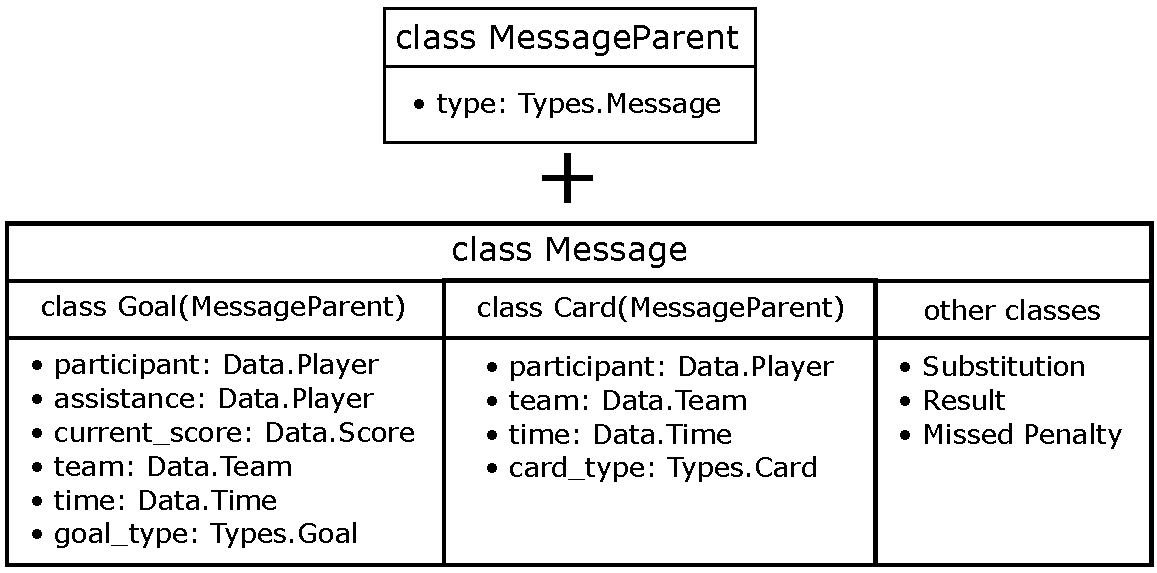
\includegraphics[width=1\textwidth]{./img/message_implementation.pdf}}
	\caption{Implementation of preverbal messages.}
	\label{fig:message}
\end{figure} 

\subsection{Sentence planner}
Last but not least is a \textit{sentence planner} module, that combines sentence aggregation, lexicalization and REG. Due to a possible low number of messages to convey, the result depends heavily on the course of the game and we do not want to leave out any of the incidents that occurred during the match. So to further simplify the process, one incident corresponds to one sentence and the sentence aggregation is not performed. Sentence aggregation as described in \ref{section:sa}, is grammatically a non-trivial operation and we leave this part as a room for improvement.

The core idea is to exploit templates, which means inserting words to express a constituent (e.g. entities to be expressed from non-verbal message) verbally in the reserved empty spot in the sentence. However, to ensure some kind of variability of the expressions as well as easy cooperating with Genja API the templates are resolved in a bit more complex way. Naming classes and variables throughout \textit{sentence planner} was difficult due to the similarities of the segments that needed to be named, therefore I first present crucial classes and reveal their overall integration later.

Firstly, the template, by its very nature, is represented as a class called \textit{\textbf{Sentence}}. \textit{Sentence} controls the structure of the sentence (ordering and selection of constituents) and allows other components of the implementation to insert various lexical items. \textit{Sentence} contains string \textit{id} to simplify the number of types and subtypes in this section. Boolean \textit{simple} says whether the expression is simple, clear, syntactically easy or the opposite: colourful, longer and more complex. Then there is a list of \textit{constituents}, which is either a hand-inserted string or \textit{Constituent}, that requires further development and will be picked later. Note that \textit{Sentence} contains an attribute \textit{msg}, but the attribute is not assigned immediately.

\begin{Verbatim}[frame=single]
class Sentence:
	id: str
	simple: bool
	constituents: List[Union[str, Constituent]]
	msg: dp.Message
\end{Verbatim}
\newpage 

Here is an example of one \textit{Sentence} initialization, which defines the easiest possibility of how to express a message that a goal was scored. Furthermore, the following table shows possible lexicalization of these constituents in English(EN) and Czech(CZ) to illustrate the principle of such a structure.\footnote{Note that the word order is not correct in the English sentence, but correct in the Czech one. My translation will mainly illustrate the process for English readers, which can lead to grammatically incorrect sentences or expressions.}

\begin{Verbatim}[frame=single]
Sentence.create(type_, subtype, True, [
  Constituent(id_='e-time', morph_params='',
  	explicit_data=Types.ExplicitEntityData.TIME),
  Constituent(id_='v-goal', morph_params='.-0-.-.-.',
  	explicit_data=None),
  Constituent(id_='e-player', morph_params='1-.-0-.-.',
  	explicit_data=Types.ExplicitEntityData.PARTICIPANT),
  Constituent(id_='w-goal', morph_params='4-.-.-.-.',
  	explicit_data=None)]))
\end{Verbatim}

\begin{center}
	\begin{tabular}{ |c|c|c|c|c| }
		\hline
		 & Time & Verb for goal &Player entity &Word for goal \\ \hline
		 & e-time & v-goal & e-player & w-goal \\ \hline
		EN &In 7th minute& scored & Ronaldo & goal. \\  
		CZ & V 7. minutě & dal & Ronaldo & gól.\\
		\hline
	\end{tabular}
\end{center}

Another class is \textit{\textbf{Constituent}} containing again \textit{id} to mark its type or subtype. In Czech multiple agreements as well as grammatical cases need to be resolved and therefore we have to store such information when creating sentence layout regardless of the lexical expression that will be inserted. All morphology attributes are stored in \textit{morph\_params} as containing case, tense, gender and ref/agr all to be then handed over to Genja API for linguistic realisation. Again, as seen in the \textit{Sentence} initialization, \textit{morph\_params} are initialized shortly using string \textit{id}.

\begin{Verbatim}[frame=single]
class Constituent:
	id: str
	morph_params: MorphParams
	explicit_data: Types.ExplicitEntityData   
	string: str   
\end{Verbatim}

Lastly, class \textit{\textbf{Template}} handles the lexicalization of every constituent.

\begin{Verbatim}[frame=single]
class Template:
	id: str
	string: str
\end{Verbatim}
\textit{Templates} can be strings, or a part of entity information can be inserted into a lexical item. \textit{Template}'s string can be defined by hand, or by function or by creating a template (by combining string and variables' string values to be inserted), which expresses the constituent. Here are examples for templates that express player entity and a word for assistance.

\begin{center}
	\begin{tabular}{ |c|c|c| }
		\hline
		\multicolumn{3}{| c |}{Entity player (e-player)} \\ \hline
		String template & EN & CZ \\ \hline
		player.full\_name & Cristiano Ronaldo  & Cristiano Ronaldo \\
		player.get\_last\_name() & Ronaldo & Ronaldo \\
		f"hráč číslo \{player.number\}" & player number 7 & hráč číslo 7 \\
		\hline
	\end{tabular}
\end{center}

\begin{center}
	\begin{tabular}{ |c|c| }
		\hline
		\multicolumn{2}{| c |}{Word assistance (w-assistance)} \\ \hline
		 EN & CZ \\ \hline
		assistance  & asistence\\
		pass & přihrávka \\
		\hline
	\end{tabular}
\end{center}

To recapitulate, class \textit{Sentence} creates templates for sentence combining and ordering numerous constituents, which are either hand-written string or represented as an internal \textit{Constituent} class. For every \textit{Constituent} an instance of the class \textit{Template} is created to then present options for expressing \textit{Constituent} in numerous ways. Note that to store a string, data to insert need to be assigned when initializing \textit{Template} (unlike \textit{Sentence}, where \textit{Message} can be added later).

To manage these objects and enable their cooperation, two handlers are created: \textit{SentenceHandler} and \textit{TemplateHandler}. \textit{Sentences} are first initialized all, then randomly shuffled and lastly grouped by their id and always using a simple sentence first. Then for each message in the article a \textit{Sentence} is picked in the order they were grouped and message is assigned to the \textit{Sentence} as attribute \textit{msg}. Once every \textit{Sentence} for a given message type is used, we pick randomly from used. This process ensures structural variability as we use the same \textit{Sentence} twice only in case that we used all of the \textit{Sentences} for a given message.

To further increase variability of the created sentences a similar process is repeated for \textit{Templates}. \textit{Templates} are randomly picked from non-used options. Once every template is present in the output, we pick random from every template ensuring we do not use the same template twice in a row. Another difference is that \textit{Templates} are first initialized all with empty values (where string is expected to be inserted) and then \textit{Template Handler} frequencies are updated to set up the initial state of \textit{Templates}. 

\subsection{Linguistic realiser}
Czech language is quite complex in terms of grammatical difficulty and therefore resolving the problem of realising chosen lexical items correctly by-hand without a proper tool performing complex morphology transformations is not efficient. This is the last step of the entire NLG process, however, without the realisation module the outputted text will not be readable. Consequently, other software was incorporated into our solution in order to perform linguistic realisation.

The system is called Genja and was provided by Geneea(see \url{https://geneea.com/}). The Genja system, which was based on Jinja, manages working with smart templates. In order to exploit templates efficiently, Genja offers tools for managing morphology and knowledge base. Note that authorization key is required in order to perform linguistic realisation. In the solution's default, the is key stored as a system environment variable to not be visible in a public GitHub repository. Without the key, the program will still run, but the linguistic realisation will not be performed and therefore the outputted text will be the intended input for Genja.

Due to the strict syntax that needs to be inputted in a Genja API request, a number of transformations need to be done. Firstly, combining plain strings in a template with morphological parameters creates a well-built input for Genja. Secondly, a json file for Genja must be created and lastly the output must be transformed from json back to string. After that the auxiliary file is deleted.

\subsection{Articles generator}
To finalise, articles generator connects modules together creating a notional one-way pipeline. 

\section{Output}
Since the lexical items and sentences' word orders are picked randomly, the output can contain a combination of expressions that are suboptimal and hard-to-read. For example when describing substitution message, realisation of two player entities can result in unappealing text, where it is not clearly visible who is the first and second player (player Vodháněl was subbed for player Kratochvíl, whose name was lexicalized as last name and first name):
\begin{center}
	\textit{V 74. minutě střídal Vodháněl Kratochvíla Miloše.(CZ)}
\end{center}
\begin{center}
	\textit{In 74th minute subbed Vodháněl Kratochvíl Miloš.(EN)}
\end{center}
Moreover, due to the international nature of the football domain, often finding grammatically correct forms of foreign names is not easy and Genja can not resolve this issue. 

To compensate for these minor problems we output multiple texts instead of just one. As said, randomness can highly affect the overall impression from the text. When generating multiple texts the probability that one output will feel better than others is then increased. The idea of generating more than one text and then picking the best result of all generated can be useful, when the quality of the outputted text can not be ensured. However, the process of selecting "the best" result can be again approached differently. The easiest solution is ,for instance, using a human evaluation. Another option is to exploit the data-driven methods and pick the version that is statistically the most similar to the texts in the acquired set of data e.g. football articles from websites. The problem of selecting "the best" option is not solved in this project. 

Here are multiple examples of lexicalization and realisation of one preverbal message containing information about player being penalized:
\begin{itemize}
	\item Message: (Type: CARD, time: 90 + 1, participant: Povazanec Jakub, team: Jablonec, card\_type: YELLOW)
	\item \textit{(EN) In the first minute of the overtime Jakub Povazanec got a yellow card.}
	\item \textit{(CZ) V první minutě nastavení druhého poločasu obdržel hráč s číslem 7 žlutou.}
	\item \textit{(CZ) Jakub Povazanec vyfasoval jednu minutu po začátku nastaveného času druhého poločasu žlutou.}
	\item \textit{(CZ) Povazanec dostal jednu minutu po začátku nastaveného času druhého poločasu žlutou kartu.}
\end{itemize}
Note that both word order and lexical expressions for the constituents differ: player (Jakub Povazanec/Povazanec/hráč s číslem 7), yellow card (žlutou/žlutou kartu) or the verb for "got"(obdržel/vyfasoval/dostal). As you can see the template system used created a variety of well-built sentences.

Now we show two examples of generated articles for the \textit{example\_match}. Messages to generate are visible from \figref{overview}, but we will state couple of first along with the title message:

\noindent\makebox[\linewidth]{\rule{\textwidth}{0.4pt}}
\textbf{Messages:}
\begin{enumerate}
	\item Type: RESULT, team\_home: Jablonec, team\_away: --Team-- Id: 804, Name: Bohemians 1905, type: AWAY, score: 3:1
	\item Type: GOAL, time: 10, participant: Trávník Michal, team: Jablonec, score: 0-0, goal\_type: Goal.PENALTY
	\item Type: GOAL, time: 44, participant: Hašek Martin, team: Bohemians 1905, score: 1-1, goal\_type: Goal.ASSISTANCE
	\item Type: SUBSTITUTION, time: 55, participant\_out: Vaníček Antonín, participant\_in: Nečas Jakub, team: Bohemians 1905
	\item ...
\end{enumerate}

\noindent\makebox[\linewidth]{\rule{\textwidth}{0.4pt}}
\textbf{Article examle No. 1/2:}
\begin{center}
\textit{Jablonec deklasoval Bohemians 1905 3:1.  }
\end{center}

\textit{V desáté minutě proměnil Trávník pokutový kop. Hráč s číslem 21 vstřelil po nahrávce Vaníčka Antonína 44 minut po začátku gól. V 55. minutě Jakub Nečas střídal za hráče s číslem 22. 62 Minut po začátku dal po nádherné kombinaci Doležal po pase Trávník Michal branku. V 69. minutě vystřídal Hašek za Michala Ševce. Hráč s číslem 17 střídal za Jana Závišku 74 minut po začátku. V 75. minutě Kratochvíl Miloš vystřídal hráče s číslem 21. Doležal Martin vsítil po asistenci Trávník gól 79 minut po začátku druhého poločasu. 87 Minut po začátku střídal Vojtěch Kubišta hráče s číslem 25. Kubišta dostal v 90. minutě žlutou kartu. Jednu minutu po začátku nastaveného času druhého poločasu vystřídal hráč s číslem 19 Doležala Martina. V první minutě nastavení druhého poločasu obdržel Povazanec žlutou. Kratochvíl Miloš vyfasoval tři minuty po začátku nastaveného času druhého poločasu žlutou kartu.}

\noindent\makebox[\linewidth]{\rule{\textwidth}{0.4pt}}
\textbf{Article example No. 2/2:}
\begin{center}
\textit{Jablonec porazil Bohemians 1905 3:1.}
\end{center}                                      

\textit{V desáté minutě proměnil Michal Trávník penaltu. Hašek dal po přihrávce Vaníčka Antonína 44 minut po začátku branku. 55 Minut po začátku druhého poločasu vystřídal hráč s číslem 10 Vaníčka. Po nádherné souhře v 62. minutě vstřelil Martin Doležal po asistenci Trávník Michal gól. 69 Minut po začátku druhého poločasu Hašek střídal za hráče s číslem 2. V 74. minutě vystřídal Jan Vodháněl za hráče s číslem 8. Miloš Kratochvíl střídal za Sobola Eduarda 75 minut po začátku. 79 Minut po začátku druhého poločasu vsítil Martin Doležal po pase Trávník branku. 87 Minut po začátku Kubišta Vojtěch vystřídal Vladimír Jovovič. Devadesát minut po začátku druhého poločasu obdržel Kubišta Vojtěch žlutou. V první minutě nastavení druhého poločasu střídal Chramosta za Martina Doležala. Povazanec dostal jednu minutu po začátku nastaveného času druhého poločasu žlutou kartu. V třetí minutě nastavení druhého poločasu vyfasoval Kratochvíl Miloš žlutou.}

\noindent\makebox[\linewidth]{\rule{\textwidth}{0.4pt}}

Football articles generated by the software are readable, fluid and somewhat variable. Outputted texts are with only a handful of mistakes (grammatical, not factual). In the 4th sentence of the first article, \textit{Trávník Michal} has an incorrect form and Genja did now manage to process this: the correct form for the 2th case is \textit{Trávníka Michala}. Same problem occurred in the second article for the name \textit{Vladimír Jovovič}. Also in the last sentence of the second article, \textit{V třetí} is not grammatically and the form should be \textit{Ve třetí} instead. 

\section{Discussion}
In this section we discuss numerous perspectives and aspects of the solution.

Several papers on the topic of football were published. First example is \cite{et1997generation} where a system of templates is incorporated in order to generate a  football report. Syntactic trees are used to implement templates. Another difference is the ordering of the messages. While our implementation orders messages chronologically, this paper does the following: first we choose the topic we have not spoken about yet e.g goals scored during the match, then we convey every message from this topic.  However, the ordering of topics can change. Consequently, we need a tool that controls the state of the generation so that we know what was or was not already mentioned (e.g. number of spectators will be mentioned in a game summary only if it was not mentioned in another topic). Context supervision is present throughout the entire generation.

Second example of the implemented NLG system about football is much newer \cite{chen2008learning}. This system generates commentaries to events on the pitch in the simulated football match. Their approach is completely non-linguistic and relies on machine learning methods. Training data consists of pairs of textual human commentary and state of the game. These two examples show two completely different approaches.

Next to discuss is the choice of the approach used in this implementation. The architecture strictly follows the division described in a modular approach exploiting the power of splitting the extremely complex NLG problem into smaller easier-to-manage segments. As discussed earlier, the raw power of data can contribute to the quality of the result and therefore the first improvement of the project would be to change the approach completely assuming you acquire the corpus data. However, a stochastic approach relies on a big amount of quality data, which are not available for me or rather their requirement would be insanely time-consuming. Moreover, this was my first NLG project. Due to my personal inexperience and lack of a large number of easily accessible data the modular approach was chosen.

Naturally, the quality of football articles created by sport journalists can hardly be matched with the quality of outputs from the \textit{FootballArticlesGenerator} software. The aim of the outputs were to be readable and form a proper Czech sentence filled with information about a football match, which was achieved. What is more, an increased variability was achieved to make text more fluid.

The complexity of the implementation was hard to deal with and not seeing the error propagation consequences the attempts of creating a fully functioning system often failed. Retrospectively, the incorporated system of "two-layered" templates (implemented as \textit{Sentence} and \textit{Template}, which both fit to the template idea) is not-optimal. As seen in initializing \textit{Templates} for \textit{Time}. Firstly, the templates are picked randomly without context, meaning we can use expressions like "Two minutes after that" and so on. Secondly, to express time more variably we would like to use another template layer connected to a set of morphological parameters to be passed to Genja, but that is not possible. The best improvement for this project would be to re-implement sentence planner and using tree structure of templates to enable having template in a template. 

Such a tree structure would then require some non-trivial design and implementation to deliver the expected result. Sentences represented as trees where nodes are either strings or templates should be pre-created  to ensure variability between the sentences used throughout the text. Then the sentence aggregation can be performed once the content of the sentences is known. Lastly, lexicalizing each template in the sentence tree by various expressions. The core problem when designing this system is interconnection between the tasks, that requires a decent amount of flexibility of the tree structure in terms of implementation. For instance, sentence aggregation can merge two of the trees together.

Consequence of the well-implemented tree structure would be a better quality article. Due to the kept approach of using templates, the level of the result would not still be near to texts produced by humans. Templates offer only a number of varieties in comparison to a complex human language. Naturally, the higher the number of templates the more variable the text will be, initially approaching the human-like level. 

In addition, the database used for this project does not contain enough information to create a somewhat complex article. Primary insufficiency is in the lack of details of incidents contained in the data. Expressing a goal is usually accompanied by a slight description of how the goal was scored: cross from the left side and top corner header, chaos in front of the net resulted in a rebound and a goal, beautiful solo play, 30 metre absolute screamer, etc. Similarly, the minor incidents like corners, shots, fouls, offsides are not present and could help when conveying more detailed text describing the true course of the game and not only major incidents. Lastly, there are no statistics and knowledge base present. When lexicalizing Cristiano Ronaldo we have only options to use number or name, while journalist would use more complicated expressions like "deadly portuguese striker", "famous CR7", "the most productive player of the Premier League or "the newest member of Manchester United squad". History of the player, current leaderboards and statistics of the season, all time best leaderboards, nicknames for entities and more are the information lacking to truly have potential to create human-like articles that would be both thrilling and informative. Not to mention incidents, which are not based on statistics, but rather on the actions that happened on the pitch. For instance, controversial calls, conflicts between players, vibes on the stadium, how well the team actually plays are all aspects that are very hard to store, classify and express, but are arguably the most interesting for a football fan besides the result of the match itself. This paragraph further proves the strength of the data-driven approach that can overcome the difficulties of lack of data by simply imitating the already existing text. For example, if a corpus contains the nickname "Blues" for "FC Chelsea" numerous times, it becomes a viable lexical expression for the FC Chelsea entity.

Even though the generated texts are well-built and correct, their usage afterwards is questionable. The popularity of sports articles lie in the tabloid style nature of the text. If they are interested in just a simple overview of the match, they use non-textual representation like \figref{overview}, which is provided online (e.g. Livesport). Moreover, the input for the program is very specific and requires an authorization key for Genja.

Personally, I am really happy with the result. The NLG system I have created is end-to-end and transforms raw data into a well-built text, which is non-trivial and variable to some extent. However, the core consequence I am glad for is the amount of knowledge I have gained in the field of NLG. I hope that somebody will use this text as a learning material when exploring the field of NLG and will find the information useful. I truly recommend this text for someone, who is preparing himself to develop his first NLG system, as the thesis often contains passages, where I struggled with the explanation of why.
































